\documentclass[11pt]{article}
\usepackage{graphicx}
\usepackage{hyperref}
\usepackage[dvipsnames, svgnames, x11names, hyperref]{xcolor}
\hypersetup{
	colorlinks,
	citecolor=Violet,
	linkcolor=Red,
	urlcolor=Blue}
%\usepackage{natbib}

\setlength{\textwidth}{6.5in}
\setlength{\headheight}{0in}
\setlength{\textheight}{8.0in}
\setlength{\hoffset}{0in}
\setlength{\voffset}{0in}
\setlength{\oddsidemargin}{0in}
\setlength{\evensidemargin}{0in}

\title{Introduction Report}

\author{Nana Ama Nyamekye Darpaah}

\begin{document}
	
	\maketitle
	
\section{Goals, Background and Plans after Graduation}

My primary goals for this course are to 
\begin{itemize}
	\item develop a healthy and productive relationship with coding as I do not particularly enjoy programming currently
	 
	\item  get better at it 
	
\end{itemize}
I took a computational math course in my second year of undergraduate studies at the University of Ghana. I also had my final year project in the area of Density Functional Theory to determine the structural and electronic properties of Potassium Niobate ($KNbO_{3}$) with first principles which included quite a lot of coding. I quickly realized I needed more practice in this area so I was an intern at Ghana Space Science and Technology Institute after graduation where I worked on a project entitled 'Classification of Galaxies using Convolutional Neural Network Techniques'. After my Master's, I plan on furthering my education and enrolling in a PhD programme related to Fusion Energy.\\
\\
\\
\begin{figure}[h]\begin{center} 
		\vspace{12pt}
		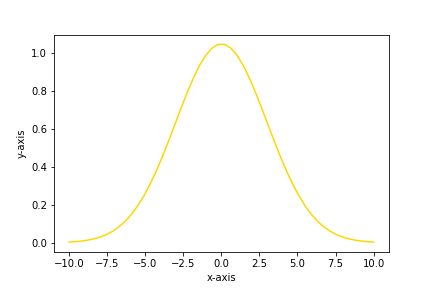
\includegraphics[width=0.99\textwidth]{gaussian.png}
		\caption{A normal distribution curve with a standard deviation of 3 and a mean of 0 over the range [-10, +10] }
		\label{fig:normal curve} 
	\end{center}
\end{figure} 


This is my GitHub link: \href{https://github.com/nnd2016/phys-ga2000.git}{Nana Ama's GitHub Link}


\end{document}